\documentclass[preprint]{revtex4-1}
\usepackage{graphicx}
\usepackage{epstopdf}
\usepackage{amsmath}
\usepackage{hyperref}
\usepackage{booktabs}
\usepackage{color}

\usepackage{SIunits}
\newcommand{\wstar}{-0.023}
\newcommand{\Qstar}{0.25}

\setlength{\tabcolsep}{10pt}

\newenvironment{sistema}%
  {\left\lbrace\begin{array}{@{}l@{}}}%
  {\end{array}\right.}


\usepackage{pgfplots}
\usepgfplotslibrary{external}
\usepgfplotslibrary{groupplots}
\usetikzlibrary{positioning}
\usetikzlibrary{plotmarks}
\usetikzlibrary{matrix}
\tikzexternalize
\tikzset{external/force remake}
\tikzset{every mark/.append style={scale=0.8}}
\pgfplotsset{every axis/.append style={small}}

\begin{document}

\begin{figure}
	\centering
	\begin{tikzpicture}[
		lab/.style={above right, text height=0.8em, text depth=0.2em, font=\bfseries}%
		]%
		\pgfplotsset{cycle list name=black white}
		\begin{axis}[%
			anchor=right of south east,%
			width=0.45\textwidth, height=0.33\textwidth, %
			xlabel=$t/\tau_B$, xmode=log,%
			ylabel={Self ISF}, ymin=0,%
			legend columns=3, reverse legend, legend style={font=\tiny, at={(1,1.03)}, anchor=south east}, %
			]
			\addplot file {LS3954.isf};
			\addplot file {LS4446.isf};
			\addplot file {LS4582.isf};
			\addplot file {LS5079.isf};
			\addplot file {go1.isf};
			\addlegendimage{legend image code/.code={\node[right] {$\phi\;\pm$};}};
			\legend{$0.497$, $0.535$, $0.540$, $0.555$, $0.575$, $0.003$};
			\node [lab] at (rel axis cs:0,0) {a};
		\end{axis}
		\begin{axis}[%
			anchor=left of south west,%
			width=0.45\textwidth, %
			xlabel=$\phi$,%
			ylabel=$\tau_\alpha/\tau_B$, ymode=log, %
			ytick pos=right, ylabel near ticks,%
			legend pos=south east,%
			cycle list={{black, mark=*},{black, mark=square}},%
			]
			%\addplot+[mark=none, forget plot, domain=0.49:0.58] {0.7874243*exp(0.32826088*x/(0.60063652-x))};
			\addplot+[mark=none, forget plot, domain=0.49:0.58] {exp(0.28970401*x/(0.59841615-x))};
			\addplot+[only marks] table[x index=0, y index=1]{xi_phi.dat};
			\addplot+[only marks] table[x index=0, y index=4]{xi_phi.dat};
			\legend{$\tau_\alpha$, $t^{dh}$};
			\node at (rel axis cs:0,1) (a) {};
			\node [lab] at (rel axis cs:0,0) {b};
		\end{axis}
		\begin{axis}[%
			tiny, at=(a), anchor=north west, %
			width=0.3\textwidth, %
			xlabel=$\phi$, xmin=0.49, xmax=0.58, xlabel near ticks,%
			xtick={0.5,0.52,...,0.6},%
			ylabel=$\xi/\sigma$, ymin=0, ymax=4.5,%
			ytick pos=right, ylabel near ticks,%
			label style={font=\tiny}, %
			legend pos=north west,%
			axis background/.style={fill=white},%
			]
			\addplot+[mark=none, forget plot, domain=0.49:0.58] {0.41158778*((0.59773962-x)/0.59773962)^(-2.0/3.0)};
			\addplot+[only marks, fill=white] table[x index=0, y index=2]{xi_phi.dat};
			\addplot+[mark=none, forget plot, domain=0.49:0.58] {0.18878182*((0.59773962-x)/0.59773962)^(-2.0/3.0)};
			\addplot+[only marks, fill=black] table[x index=0, y index=3]{xi_phi.dat};
			\legend{$\xi_u$ dynamical, $\xi_6$ structural};
		\end{axis}
	\end{tikzpicture}
	\caption{\textbf{Dynamics of the system.} {\bf a,} Decay of the self-intermediate scattering function computed from the positions for several volume fractions. {\bf b,} The structural relaxation time $\tau_\alpha$ and the characteristic time of the dynamic heterogeneity $t^{dh}$ scaled by the Brownian time $\tau_B$ as a function of $\phi$. The solid curve is the VFT fit of $\tau_\alpha$. Inset: Dynamical ($\xi_u$) and structural correlation length ($\xi_6$). Solid curves are power-law fits (see text).}
	\label{fig:vft}
\end{figure}

\begin{figure}
	\begin{tikzpicture}[
		lab/.style={below right, text height=0.8em, text depth=0.2em, font=\bfseries}%
		]%
		\pgfplotsset{
			extra tick style={grid=major},%
			every axis/.append style={%
				height=0.4\textwidth,
				ymin=0,ymax=0.6,%
				extra y ticks={\Qstar}, extra y tick labels={},%
				enlargelimits=false,axis on top,
				colormap={bw}{gray(0cm)=(1); gray(1cm)=(1); gray(10cm)=(0)},%
				colorbar sampled,%
				},%
		}
		\begin{groupplot}[
			group style={
				group size=2 by 1,%
				yticklabels at=edge left,%
				horizontal sep=0pt,%
				},%
			anchor=below south west,%
			width=0.45\textwidth,%
			xtick scale label code/.code={},%
			colorbar horizontal, colorbar style={%
				samples=6, xtick={ 0.20,0.4,0.6, 0.8},% 
				extra y ticks={},%
				/pgfplots/colorbar shift/.style={yshift=0.3cm},
				at={(parent axis.north)}, anchor=below south, width=0.9*\pgfkeysvalueof{/pgfplots/parent axis width},
				xticklabel pos=upper,%
				label style={font=\footnotesize},
				},%
			]
		\nextgroupplot[%
			ylabel={$Q_6$}, xlabel=$Q_4$,%
			xmin=0,xmax=0.22,%
			colorbar style={%
				xlabel={per units of $Q_4\cdot Q_6$},% 
				xticklabels={$10^{1}$, $10^{2}$, $10^{3}$, $10^{4}$},%
				},%
			xticklabel={$\pgfmathprintnumber[fixed,precision=2]{\tick}$}
			]
		\addplot graphics
		[xmin=0,xmax=0.2,ymin=0,ymax=0.6]
		{Q4Q6go1};
		\node [lab] at (rel axis cs:0,1) {a};
		\node [below] at (axis cs:0.1909, 0.5745) {\textsc{fcc}};
		\node [below] at (axis cs:0.0972222, 0.484762) {\textsc{hcp}};
		\node [below] at (axis cs:0.0363696, 0.510688) {\textsc{bcc}};
		\draw[->, white,thick] (axis cs:0.05, 0.15) to [out=60, in=220] (axis cs:0.125, 0.4);
		
		\nextgroupplot[%
			xlabel=$10^3 \cdot w_4$, %
			xmin=-0.002,xmax=0.002,%
			xtickmin=-0.0015,%
			extra x ticks=0, extra x tick labels={},
			colorbar style={%
				xlabel={per units of $w_4\cdot Q_6$},% 
				xticklabels={$10^{3}$, $10^{4}$, $10^{5}$, $10^{6}$},%
				},%
			]
		\addplot graphics
		[xmin=-0.002,xmax=0.002,ymin=0,ymax=0.6]
		{w4Q6go1};
		\node [lab] at (rel axis cs:0,1) {b};
		\node [below] at (axis cs:-0.00067221, 0.5745) {\textsc{fcc}};
		\node [below] at (axis cs:7.47E-05, 0.484762) {\textsc{hcp}};
		%\node [below] at (axis cs:-0.01274716, 0.510688) {\textsc{bcc}};
		\node [above] at (axis cs:0.0015, \Qstar) {\footnotesize{$Q_6^*$}};
		\draw[->, white,thick] (axis cs:0, 0.15) to [out=120, in=280] (axis cs:-0.0005, 0.4);
		\draw[->, white,thick] (axis cs:0, 0.15) to (axis cs:7E-05, 0.35);
		
		\end{groupplot}
		
		\begin{groupplot}[
			group style={
				group size=2 by 1,%
				yticklabels at=edge left,%
				horizontal sep=0pt,%
				},%
			anchor=above north west,%
			width=0.38\textwidth,%
			xlabel=$10^2 \cdot w_6$,%
			xmin=-0.052,xmax=0.01,%
			extra x ticks={\wstar, -0.00782},%
			extra x tick labels={,},%
			xtick scale label code/.code={},%
			colorbar right, colorbar style={%
				samples=6, ytick={ 0.20,0.4,0.6, 0.8},% 
				yticklabels={$10^{1}$, $10^{2}$, $10^{3}$, $10^{4}$},%
				ylabel={per units of $w_6\cdot Q_6$},%
				extra x ticks={},%
				extra y ticks={},%
				label style={font=\footnotesize},
				},%
			]
		
		\nextgroupplot[ylabel={$Q_6$}, xtickmax=0,]
		\addplot graphics
		[xmin=-0.052,xmax=0.052,ymin=0,ymax=0.6]
		{u6Q6go1_scale};
		\node [lab] at (rel axis cs:0,1) {c};
		\node at (axis cs:\wstar,0.6) (a) {};
		\node at (axis cs:-0.00782,0.6) (b) {};
		\node [below] at (axis cs:-0.0026, 0.5745) {\textsc{fcc}};
		\node [below, right] at (axis cs:-0.052, 0.05) {\textsc{Ico}};
		\draw[->, white,thick] (axis cs:-0.001, 0.15) to [out=90, in=275] (axis cs:-0.0015, 0.33);
		\draw[->, white,thick] (axis cs:-0.001, 0.15) to [out=180, in=30] (axis cs:-0.025, 0.12);
		
		\nextgroupplot
		\addplot graphics
		[xmin=-0.052,xmax=0.052,ymin=0,ymax=0.6]
		{u6Q6phi3954_scale};
		\node [lab] at (rel axis cs:0,1) {d};
		\node [above] at (axis cs:-0.04, \Qstar) {\footnotesize{$Q_6^*$}};
		%\node [anchor=north east] at (rel axis cs:1, 1) {\footnotesize{$\phi = 0.497 \pm 0.03$}};
		\node [left] at (axis cs:\wstar,0.4) {\footnotesize $w_6^*$};
		\node [right] at (axis cs:-0.00782,0.4) {\footnotesize $w_6^{dod}$};
		
		\end{groupplot}
	\end{tikzpicture}
	\caption{Population of local structures function of \textsc{boo}. (a-c) For our deepest supercooled sample ($\phi=0.575\pm 0.03$) in the $(Q_4,Q_6)$-plane (a), $(w_4,Q_6)$-plane (b) and $(w_6,Q_6)$-plane (c). (d) is the same as (c) but for a liquid near the freezing point ($\phi = 0.497 \pm 0.03$). Colour represent the probability to find the structure (log scale). The arrows stress the ordering tendencies: the tendency toward \textsc{fcc} is always visible, but a tendency toward \textsc{hcp} can be distinguished in (b) and the tendency toward icosahedral order is visible in (c).}
	\label{fig:maps}
\end{figure}


\begin{figure}
	\begin{tikzpicture}[
		lab/.style={text height=0.8em, text depth=0.2em, font=\bfseries}%
		]%
		\begin{axis}[%
			anchor=below south,%
			width=0.5\textwidth,%
			height=0.5\textwidth,%
			ylabel=$Q_6$,%
			ymin=0,ymax=0.6,%
			xlabel=$10^2 \cdot w_6$,%
			xmin=-0.052,xmax=0.01,%
			xtick scale label code/.code={},%
			enlargelimits=false,axis on top,
			colormap={sd}{color(0cm)=(black) rgb(1cm)=(0.5, 0, 0) rgb(2cm)=(1, 0.5, 0) color(3cm)=(yellow) rgb(4cm)=(0.5, 0.75, 1) rgb(5cm)=(0.5, 0.75, 1)},%
			extra x ticks={\wstar, -0.00782},%
			extra x tick style={grid=major,	tick label style={anchor=south west}},%
			extra x tick labels={,},%
			extra x tick style={grid=major},
			extra y ticks={\Qstar},
			extra y tick style={grid=major},
			extra y tick labels={},%
			colorbar sampled, colorbar style={%
				samples=5, ytick={ 0, 0.25, 0.5, 0.75},% 
				yticklabels={$0$, $0.5$, $1$, $1.5$},%
				ylabel=${\Delta r^2(w_6, Q_6, t^{dh})}/{\langle\Delta r^2(t^{dh}) \rangle}$,%
				extra x ticks={},%
				yticklabel pos=right,%
				label style={font=\footnotesize},
				},%
			]
			\addplot graphics [xmin=-0.052,xmax=0.052,ymin=0,ymax=0.6]{sd_u6Q6_go1_color};
			\node [lab, anchor=north west] at (rel axis cs:0,1) {a};
			\node [above] at (axis cs:-0.04, \Qstar) {\footnotesize{$Q_6^*$}};
			\node [anchor=west] at (rel axis cs:0, 0.8) {\footnotesize{$\phi = 0.575 \pm 0.03$}};
			\node [left] at (axis cs:\wstar,0.55) {\footnotesize $w_6^*$};
			\node [left] at (axis cs:-0.00782,0.55) {\footnotesize $w_6^{dod}$};
			\node [below] at (axis cs:-0.0026, 0.5745) {\textsc{fcc}};
			\node [below, right] at (axis cs:-0.052, 0.05) {\textsc{Ico}};
		\end{axis}
		\pgfplotsset{every axis plot/.append style={only marks}}
		\begin{groupplot}[%
			group style={
				group size=2 by 2,%
				yticklabels at=edge left,%
				horizontal sep=0pt,%
				},%
			anchor=outer north east,%
			width=0.5\textwidth,%
			ymin=0, ymax=1.5,%
			extra x tick style={grid=major,	tick label style={anchor=south west}},%
			extra y ticks={1},%
			extra y tick style={grid=major,	tick label style={anchor=south west}}, extra y tick labels={},%
			%legend columns=5,%
			legend style={
				font=\footnotesize,
				%at={(1,1)}, anchor=south,%
				at={(1,1)}, anchor=north east
				},%
			]
			\nextgroupplot[%
				xlabel=$10^2 \cdot w_6$, xmin=-0.0521089193, xmax=0.01,%
				xtickmax={0},%
				xtick scale label code/.code={},%
				ylabel=${\Delta r^2(w_6,Q_6,t^{dh})}/{\langle\Delta r^2(t^{dh}) \rangle}$,
				extra x ticks={\wstar, -0.00782}, extra x tick labels={$w_6^*$,$w_6^{dod}$},%
				extra y tick labels={bulk}
				]
			
			%\addplot table[x index=0, y expr={\thisrowno{1}/\thisrowno{2}}]{sd_nb_u6_phi3954.txt};
			\addplot table[x index=0, y expr={\thisrowno{1}/\thisrowno{2}}]{sd_nb_u6_phi4446.txt};
			\addplot table[x index=0, y expr={\thisrowno{1}/\thisrowno{2}}]{sd_nb_u6_phi5079.txt};
			\addplot table[x index=0, y expr={\thisrowno{1}/\thisrowno{2}}]{sd_nb_u6_go1.txt};
			\addplot+[domain=-0.0521089193:0.01, sharp plot, no markers] {9.34701 * x + 1.03764};
			\draw[->, thick] (rel axis cs:0.2, 0.9) to (rel axis cs:0, 0.9);
			\node[right] at (rel axis cs:0.2, 0.9) {\footnotesize Icosahedron};
			\node [lab, anchor=south west] at (rel axis cs:0,0) {b};
			
			\nextgroupplot[%
				xlabel=$Q_6$, xmin=0, xmax=0.5745,%
				extra x ticks={\Qstar}, extra x tick labels={$Q_6^*$},%				
				]
			\addlegendimage{legend image code/.code={\node[right] {$\phi\;\pm$};}};
			\legend{$0.003$,%$0.497$, 
				$0.535$, $0.555$, $0.575$};
			%\addplot table[x index=0, y expr={\thisrowno{1}/\thisrowno{2}}]{sd_nb_Q6_3954.txt};
			\addplot+[domain=0.05:0.3, sharp plot, no markers, forget plot] {-0.76 * x + 1.1};
			\addplot table[x index=0, y expr={\thisrowno{1}/\thisrowno{2}}]{sd_nb_Q6_4446.txt};
			%\addplot+[domain=0.05:0.3, sharp plot, no markers, forget plot] {1.09-1.18*x+8.95*x^2-38*x^3};
			\addplot+[smooth, no markers, forget plot] coordinates {(0.08, 1.04) (0.2, 0.92) (0.32, .62)};
			\addplot table[x index=0, y expr={\thisrowno{1}/\thisrowno{2}}]{sd_nb_Q6_5079.txt};
			\addplot+[smooth, no markers, forget plot] coordinates {(0.08, 1.23) (0.1, 1.22) (0.15, 1.07) (0.25, 0.65) (0.35, 0.33) (0.45, 0.18) (0.5, 0.15)};
			\addplot table[x index=0, y expr={\thisrowno{1}/\thisrowno{2}}]{sd_nb_Q6_go1.txt};
			\draw[->, thick] (rel axis cs:0.8, 0.45) to (rel axis cs:1, 0.45);
			\node[left] at (rel axis cs:0.8, 0.45) {\footnotesize \textsc{fcc}};
			\node [lab, anchor=south west] at (rel axis cs:0,0) {c};
		\end{groupplot}
	\end{tikzpicture}
	\caption{{\bf Bond order mobility.} (a) Normalised mobility in the $(w_6, Q_6)$-plane for our most deeply supercooled sample. The colour scale is saturated at $1.5$ times the bulk mean square displacement. (b-c) Normalised mobility for icosahedral and crystalline order parameters respectively. Bulk mean square displacement is at 1. Perfect structures are on the edge of each plot. The line is a guide for the eye stressing the collapse of the $w_6$-mobility at all volume fractions. Scattering away from the lines is due to poor averaging.}
	\label{fig:msd_Q6_w6}
\end{figure}


\begin{figure}
	\centering
	\begin{tikzpicture}[%
		pic3d/.style={inner sep=0}, %
		lab/.style={below left=0.002\textwidth and 0.005\textwidth, text height=0.8em, text depth=0.2em, font=\bfseries},%
		arr/.style={<->, thick, yellow!75!black}%
		]%
	\definecolor{turquoise}{rgb}{0.678431,0.917647,0.917647}
	\node[right=0.01\textwidth, pic3d] (all) {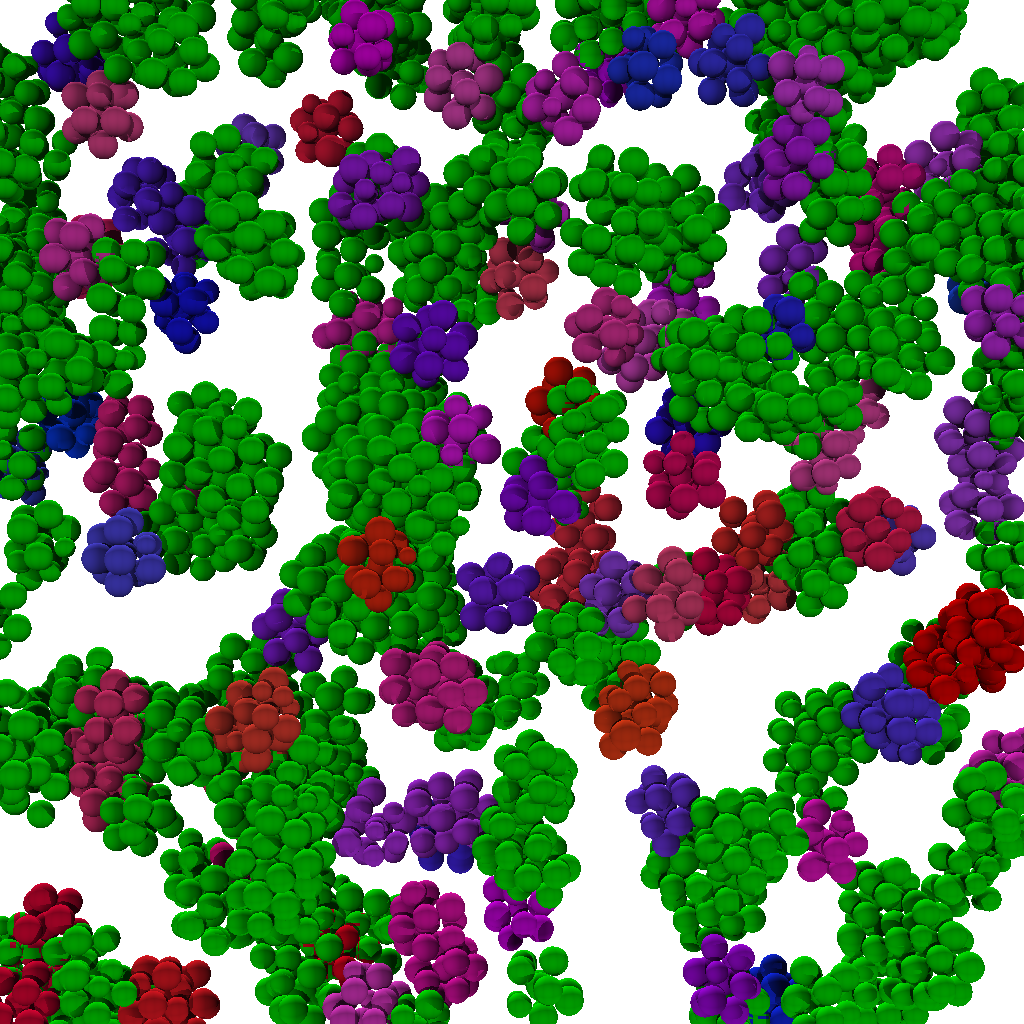
\includegraphics[width=0.48\textwidth]{mrco_ico_scale_go1-0023.png}};
	\node[below=0.01\textwidth, pic3d] at (all.south) (dyn) {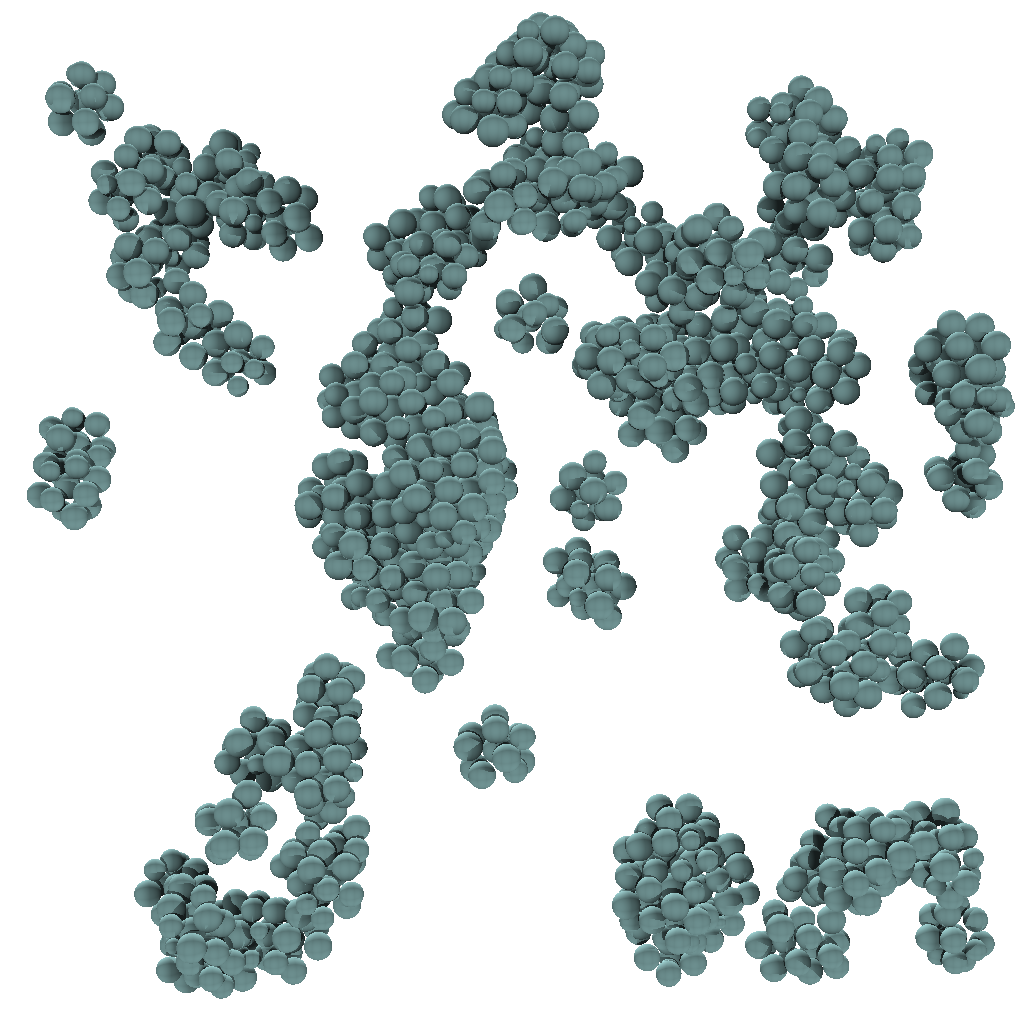
\includegraphics[width=0.48\textwidth]{cgsd_2tau.png}};
	\node[left=0.01\textwidth, pic3d] at (dyn.west) (mrco) {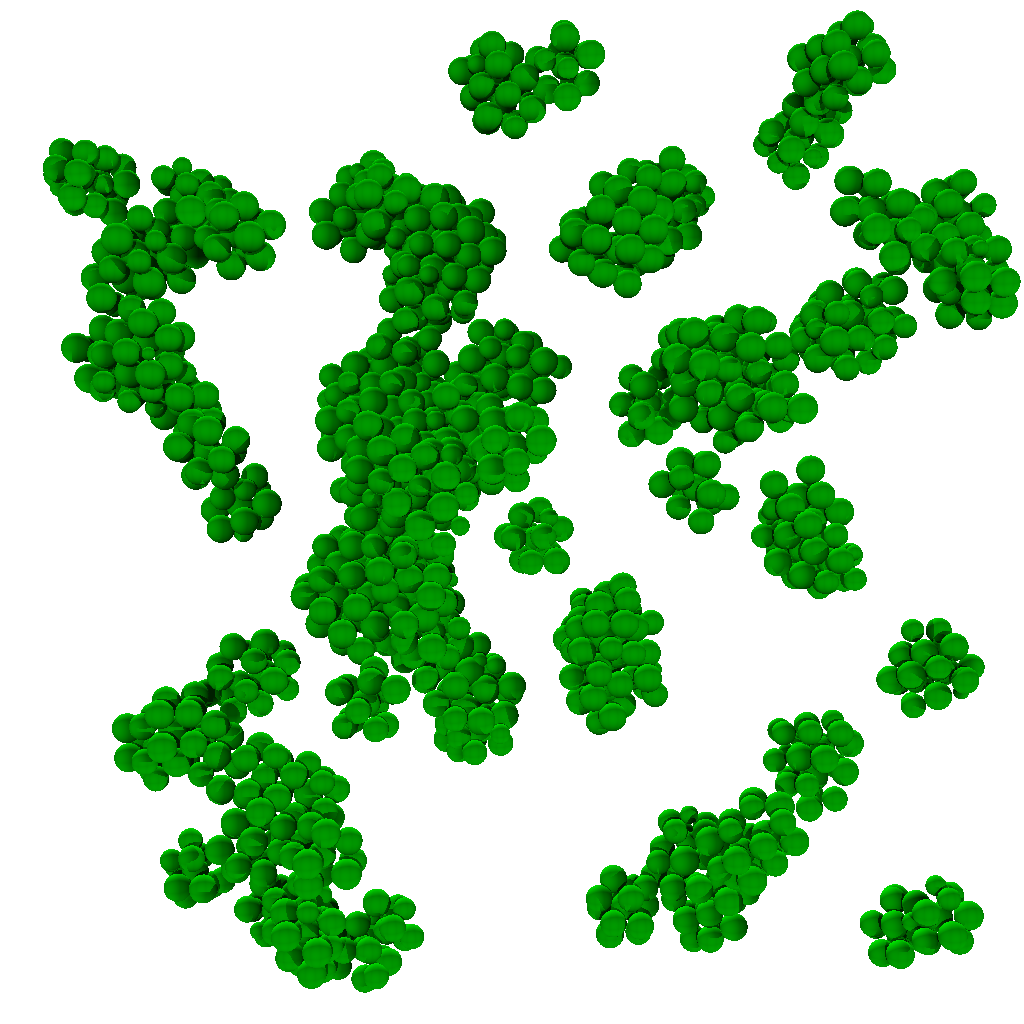
\includegraphics[width=0.48\textwidth]{mrco24_scale_go1_t040_t048.png}};
	\draw [help lines, step=0.12\textwidth, shift=(mrco.south west)] (0, 0) grid (0.48\textwidth, 0.48\textwidth);
	\draw [help lines, step=0.12\textwidth, shift=(dyn.south west)] (0, 0) grid (0.48\textwidth, 0.48\textwidth);
	\matrix[%
		matrix anchor=east, draw, font=\footnotesize,% 
		column 1/.style={text height=0.8em, text depth=0.2em},%
		column 2/.style={circle, shade, inner sep=0.008\textwidth},%
		] (l)
	{
		\node{Icosahedra}; & \node[ball color=red!50!blue] (b2) {};\node[ball color=red!75!black, left] at (b2.west) {}; \node[ball color=blue!75!black, right] at (b2.east) {};\\
		\node{Crystal-like}; & \node[ball color=green!66!black] {}; \\
		\node{Slow}; & \node[ball color=turquoise!75!black] {}; \\
	};
	\node[above left=0.01\textwidth, pic3d] at (l.west) (one_ico) {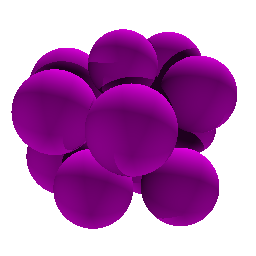
\includegraphics[width=0.22\textwidth]{one_ico.png}};
	\node[right=0.01\textwidth] at (one_ico.east){$w_6=w_6^*$};
	\node[below left=0.01\textwidth, pic3d] at (l.west) (one_mrco) {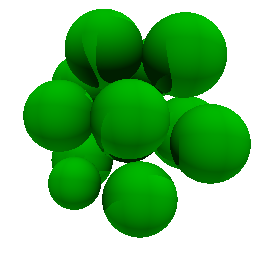
\includegraphics[width=0.22\textwidth]{one_mrco.png}};
	\node[right=0.01\textwidth] at (one_mrco.east) {$Q_6=Q_6^*$};
	\node [lab] at (one_ico.north east) {a};
	\node [lab] at (one_mrco.north east) {b};
	\node [lab] at (all.north east) {c};
	\node [lab] at (mrco.north east) {d};
	\node [lab] at (dyn.north east) {e};
	\end{tikzpicture}
	\caption{\textbf{Computer reconstruction from confocal microscopy coordinates in our most deeply supercooled sample.} Depth is $\sim 12\sigma$. Only particles of interest and their neighbours are displayed. Each particle is plotted with its real radius.  Example of \textbf{a} distorted icosahedron and \textbf{b} crystal-like cluster at the respective threshold values. \textbf{c,} A typical configuration of bond ordered particles. Two icosahedral particle are shown in the same shade if they belong to the same cluster. If a particle is neighbouring both kind of structures, it is displayed as icosahedral. \textbf{d,} Crystal-like particles alone (the order parameter was averaged over $t^{dh}/2$). \textbf{e,} Slow particles (see text). Due to particles going in and out of the field of view, the edges of \textbf{d} and \textbf{e} were not accurate and have been removed.}
	\label{fig:3D}
\end{figure}

\begin{figure}
	\centering
	\begin{tikzpicture}[%
		pic3d/.style={inner sep=0}, %
		lab/.style={below left=0.002\textwidth and 0.005\textwidth, text height=0.8em, text depth=0.2em, font=\bfseries},%
		]%
	\node[above left=0.01\textwidth, pic3d] (X) {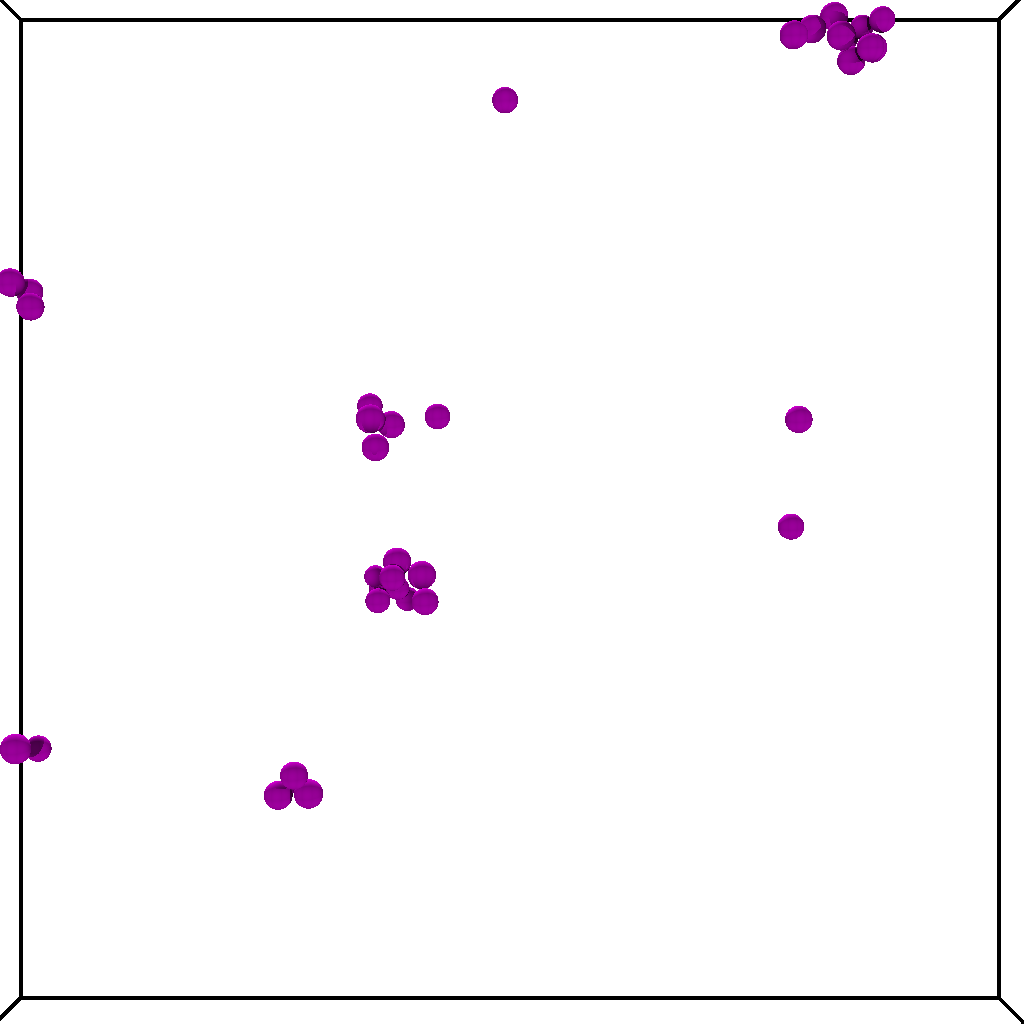
\includegraphics[width=0.48\textwidth]{X_go1.png}};
	\node[above right=0.01\textwidth, pic3d] (mrco) {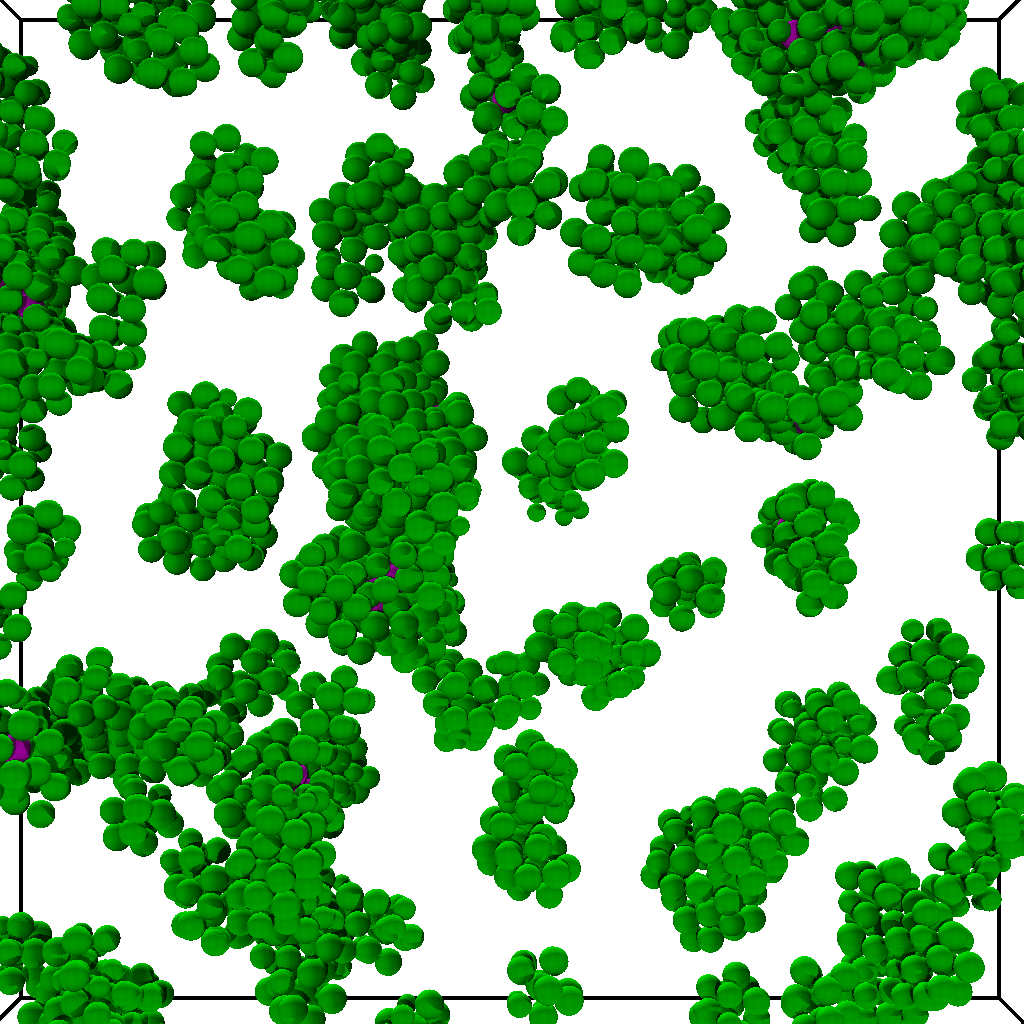
\includegraphics[width=0.48\textwidth]{X_mrco_go1.png}};
	\matrix[%
		above left=0.1\textwidth of X.south east, matrix of nodes, ampersand replacement=\&,%
		draw,%
		%every even column/.style={text height=0.8em, text depth=0.2em},%
		every odd column/.style={circle, shade, inner sep=0.25em, above},%
		]{%
		|[ball color=magenta]| \& Crystal \\
		%|[ball color=cyan]| \& Crystal neighbour \&
		|[ball color=green!66!black]| \& Crystal-like \\
	};
	\node [lab] at (X.north east) {a};
	\node [lab] at (mrco.north east) {b};
	\end{tikzpicture}
	\caption{\textbf{Particles with more than $7$ crystalline bonds.} Particles with $Q_6>Q_6^*$ and their neighbours are also plotted in \textbf{b} for comparison. Crystalline particles are always included in high $Q_6$ regions. However, the fluctuations of the crystal-like order cannot be reduced to sub-critical nucleation.}
	\label{fig:X_3D}
\end{figure}

\end{document}